\newpage
\section{Variational Diffusion Models}
\label{sec: variational diffusion models}
%
\begin{figure}[!t]
    \centering
    \hfill
    \begin{subfigure}{.24\columnwidth}
        \centering
        \begin{tikzpicture}[thick,scale=1, every node/.style={scale=1}]
            \node[obs] (x) {$\mathbf{x}$};
            \node[latent, below=15pt of x] (zt) {$\mathbf{z}_T$};
            \draw node[draw=none, scale=0.75, below=6pt of zt] (z3) {\hspace{0.5pt}\rotatebox{90}{$\mathbf{\cdots}$}};
            \node[latent, below=13pt of z3] (z2) {$\mathbf{z}_2$};
            \node[latent, below=15pt of z2] (z1) {$\mathbf{z}_1$};
            \edge[-{Latex[scale=1.0]}]{x}{zt}
            \edge[-]{zt}{z3}
            \edge[-{Latex[scale=1.0]}]{z3}{z2}
            \edge[-{Latex[scale=1.0]}]{z2}{z1}
            \draw [-{Latex[scale=1.0]}] (x) to [out=225,in=135] (z2);
            \draw [-{Latex[scale=1.0]}] (x) to [out=225,in=135] (z1);
            \node[latent, draw=none, right=-4pt of x, yshift=-16pt] (eq1) {$q(\mathbf{z}_T \mid \mathbf{x})$};
            \node[latent, draw=none, right=-4pt of z2, yshift=-16pt] (eq2) {$q(\mathbf{z}_1 \mid \mathbf{z}_2, \mathbf{x})$};
            \node[latent, draw=none, right=-4pt of z3, xshift=6pt, yshift=-0pt] (eq3) {$q(\mathbf{z}_{t-1} \mid \mathbf{z}_{t}, \mathbf{x})$};
        \end{tikzpicture}
        \caption{Top-down Hierarchy}
    \end{subfigure}
    \hfill
    \begin{subfigure}{.2\columnwidth}
        \centering
        \begin{tikzpicture}[thick,scale=1, every node/.style={scale=1}]
            \node[obs] (x) {$\mathbf{x}$};
            \node[latent, below=15pt of x] (zt) {$\mathbf{z}_T$};
            \draw node[draw=none, scale=0.75, below=6pt of zt] (z3) {\hspace{0.5pt}\rotatebox{90}{$\mathbf{\cdots}$}};
            \node[latent, below=13pt of z3] (z2) {$\mathbf{z}_2$};
            \node[latent, below=15pt of z2] (z1) {$\mathbf{z}_1$};
            \edge[-]{zt}{z3}
            \edge[-{Latex[scale=1.0]}]{z3}{z2}
            \edge[-{Latex[scale=1.0]}]{z2}{z1}
            \draw [-{Latex[scale=1.0]}] (x) to [out=225,in=135] (z2);
            \draw [-{Latex[scale=1.0]}] (x) to [out=225,in=135] (z1);
            \draw [densely dashed, -{Latex[scale=1.0]}] (zt) to [out=45,in=-45] (x);
            \draw [densely dashed, -{Latex[scale=1.0]}] (z2) to [out=45,in=-45] (x);
            \draw [densely dashed, -{Latex[scale=1.0]}] (z1) to [out=45,in=-45] (x);
        \end{tikzpicture}
        \caption{Diffusion Model}
    \end{subfigure}
    \hfill
    \begin{subfigure}{.26\columnwidth}
        \centering       
        \begin{tikzpicture}[thick,scale=1, every node/.style={scale=1}]
            \node[latent] (zt) {$\mathbf{z}_T$};
            \draw node[draw=none, scale=0.75, below=6pt of zt] (z3) {\hspace{0.5pt}\rotatebox{90}{$\mathbf{\cdots}$}};
            \node[latent, below=13pt of z3] (z2) {$\mathbf{z}_2$};
            \node[latent, below=15pt of z2] (z1) {$\mathbf{z}_1$};
            \edge[-]{zt}{z3}
            \edge[-{Latex[scale=1.0]}]{z3}{z2}
            \edge[-{Latex[scale=1.0]}]{z2}{z1}
            \node[latent, draw=none, right=-4pt of z2, yshift=-16pt] (eq2) {$q(\mathbf{z}_1 \mid \mathbf{z}_2, \mathbf{d}_1)$};
            \node[latent, draw=none, right=-4pt of z3, xshift=6pt, yshift=-0pt] (eq3) {$q(\mathbf{z}_{t-1} \mid \mathbf{z}_t, \mathbf{d}_t)$};

            \node[latent, draw=none, left=15pt of zt] (dt) {$\mathbf{d}_T$};
            \draw node[draw=none, scale=0.75, below=13pt of dt] (d3) {\hspace{0.5pt}\rotatebox{90}{$\mathbf{\cdots}$}};
            \node[latent, draw=none, left=15pt of z2] (d2) {$\mathbf{d}_2$};
            \node[latent, draw=none, left=15pt of z1] (d1) {$\mathbf{d}_1$};
            \node[obs, below=15pt of d1] (x) {$\mathbf{x}$};
            
            \edge[-{Latex[scale=1.0]}]{d3}{dt}
            \edge[-]{d2}{d3}
            \edge[-{Latex[scale=1.0]}]{d1}{d2}
            \edge[-{Latex[scale=1.0]}]{x}{d1}
            \edge[-{Latex[scale=1.0]}]{dt}{zt}
            \edge[-{Latex[scale=1.0]}]{d2}{z2}
            \edge[-{Latex[scale=1.0]}]{d1}{z1}
        \end{tikzpicture}
        \caption{HVAE Inference Model}
    \end{subfigure}
    \hfill
    \begin{subfigure}{.26\columnwidth}
        \centering
        \begin{tikzpicture}[thick,scale=1, every node/.style={scale=1}]
            \node[latent, below] (zt) {$\mathbf{z}_T$};
            \draw node[draw=none, scale=0.75, below=6pt of zt] (z3) {\hspace{0.5pt}\rotatebox{90}{$\mathbf{\cdots}$}};
            \node[latent, below=13pt of z3] (z2) {$\mathbf{z}_2$};
            \node[latent, below=15pt of z2] (z1) {$\mathbf{z}_1$};
            \node[obs, below=15pt of z1] (x) {$\mathbf{x}$};
            \node[latent, draw=none, left=15pt of z1] (d1) {${\mathbf{d}}_1$};
            \node[latent, draw=none, left=15pt of z2] (d2) {${\mathbf{d}}_2$};

            \draw node[draw=none, scale=0.75, left=4pt of z3] (d3) {\hspace{0.5pt}\rotatebox{55}{$\mathbf{\cdots}$}};
            
            \edge[-]{zt}{z3}
            \edge[blue,-]{zt}{d3}
            \edge[blue,-{Latex[scale=1.0]}]{d3}{d2}
            \edge[blue, -{Latex[scale=1.0]}]{z2}{d1}
        
            \edge[-{Latex[scale=1.0]}]{z3}{z2}
            \edge[-{Latex[scale=1.0]}]{z2}{z1}
            \edge[-{Latex[scale=1.0]}]{z1}{x}
            \edge[-{Latex[scale=1.0]}]{d1}{z1}
            \edge[-{Latex[scale=1.0]}]{d2}{z2}

            \node[latent, draw=none, right=-4pt of z2, yshift=-16pt] (eq2) {$q(\mathbf{z}_1 \mid \mathbf{z}_2, \mathbf{d}_1)$};
            \node[latent, draw=none, right=-4pt of z3, xshift=6pt, yshift=-0pt] (eq3) {$q(\mathbf{z}_{t-1} \mid \mathbf{z}_{t}, \mathbf{d}_t)$};
        \end{tikzpicture}
        \caption{Reverse Process}
    \end{subfigure}
    \hfill
    \caption{Probabilistic graphical models of HVAEs and diffusion models. \textbf{(a)} The general top-down hierarchical latent variable model. \textbf{(b)} The top-down model used to specify diffusion models, where $q(\mathbf{z}_T \mid \mathbf{x}) = q(\mathbf{z}_T)$ by construction. Here the posterior $q(\mathbf{z}_{1:T} \mid \mathbf{x})$ is a fixed noising process, so the modelling task is bottom-up prediction of $\mathbf{x}$ from each $\mathbf{z}_t$, i.e. denoising (dashed lines). \textbf{(c)} The top-down model used for posterior inference in HVAEs. It consists of a deterministic bottom-up pass to compute $\mathbf{d}_1,\dots,\mathbf{d}_T$, followed a stochastic top-down pass to compute $\mathbf{z}_T,\dots,\mathbf{z}_1$. \textbf{(d)} The reverse process of a diffusion model, i.e. the generative model. The main differences compared to (c) are that here the deterministic variables $\mathbf{d}_{T-1},\dots,\mathbf{d}_1$ do not depend on $\mathbf{x}$ nor have their own hierarchical dependencies. Further, the {\color{blue}blue} lines represent a denoising model $\hat{\mathbf{x}}_{\boldsymbol{\theta}} :\mathbf{z}_t \to \mathbf{d}_t$ which is \textit{shared} across the hierarchy.
    }
    \label{fig: hvae2}
\end{figure}
%
A diffusion probabilistic model~\citep{sohl2015deep} can be understood as a hierarchical VAE with a particular choice of inference and generative model. Like HVAEs, diffusion models are deep latent variable models that maximize the variational lower bound of the log-likelihood of the data (i.e. the ELBO). Diffusion models were largely inspired by ideas from statistical physics rather than variational Bayesian methods, so they come with a different set of modelling choices and advantages. The general idea behind diffusion models is to define a \textit{fixed} forward (inference) diffusion process that converts any complex data distribution into a tractable distribution, and then learn a generative model that reverses this diffusion process. Figure~\ref{fig: hvae2} compares diffusion models with (top-down inference) HVAEs.

Diffusion probabilistic models have the following distinctive properties:
\begin{enumerate}[(i)]
    \item The joint posterior $q(\mathbf{z}_{1:T} \mid \mathbf{x})$ is fixed rather than learned from observed data. This amounts to having a fixed encoder defining a \textit{Gaussian diffusion process} of the data;
    \item Each latent variable $\mathbf{z}_t$ has the same dimensionality as the input data $\mathbf{x}$;
    \item The aggregate posterior $q(\mathbf{z}_T)$ is equal to the prior $p(\mathbf{z}_T)$ by construction;
    \item The functional form of the inference model is identical to that of the generative model. This corresponds exactly to the top-down inference model structure used in HVAEs;
    \item A single neural network is shared across all levels of the latent variable hierarchy, and each layer can be trained without having to compute the preceding ones;
    \item They maximize a particular \textit{weighted} objective which seems to better align with human perception by suppressing modelling effort on imperceptible details.
\end{enumerate}
%
\begin{figure}[!t]
    \hfill
    \begin{subfigure}{.32\columnwidth}
        \centering
        \begin{tikzpicture}[thick,scale=1, every node/.style={scale=1}]
            \node[obs] (x) {$\mathbf{x}$};
            \node[latent, above=20pt of x] (z1) {$\mathbf{z}_1$};
            \node[latent, above=20pt of z1] (z2) {$\mathbf{z}_{2}$};
            \draw node[draw=none, scale=0.8, above=9pt of z2] (z3) {\hspace{0.5pt}\rotatebox{90}{$\mathbf{\cdots}$}};
            \draw [-{Latex[scale=1.0]}] (x) to [out=45,in=-45] (z2);
            \node[latent, above=9pt of z3] (zt) {$\mathbf{z}_T$};
            \edge[-{Latex[scale=1.0]}]{x}{z1}
            \node[rectangle, draw=none, fill=white, scale=1, above=2pt of x, xshift=-12pt] (eq1) {$\alpha_1$};
            \draw [-{Latex[scale=1.0]}] (x) to [out=45,in=-45] (zt);
            \node[rectangle, draw=none, fill=white, scale=1, right=22pt of z2, yshift=-13pt] (eq2) {$\alpha_T$};
            \node[rectangle, draw=none, scale=1, left=15pt of zt] (nt) {$\mathcal{N}\big(0, \sigma^2_T\mathbf{I}\big)$};
            \node[rectangle, draw=none, scale=1, left=15pt of z2] (n2) {$\mathcal{N}\big(0, \sigma^2_2\mathbf{I}\big)$};
            \node[rectangle, draw=none, scale=1, left=15pt of z1] (n1) {$\mathcal{N}\big(0, \sigma^2_1\mathbf{I}\big)$};
            \edge[-{Latex[scale=1.0]}]{nt}{zt}
            \edge[-{Latex[scale=1.0]}]{n2}{z2}
            \edge[-{Latex[scale=1.0]}]{n1}{z1}
            \node[rectangle, draw=none, fill=white, scale=1, right=11pt of z1, yshift=-1pt] (eq2) {$\alpha_2$};
        \end{tikzpicture}
        \caption{Gaussian Diffusion}
        \label{fig: gd}
    \end{subfigure}
    \hfill
    \begin{subfigure}{.32\columnwidth}
        \centering
        \begin{tikzpicture}[thick,scale=1, every node/.style={scale=1}]
            \node[obs] (x) {$\mathbf{x}$};
            \node[latent, above=20pt of x] (z1) {$\mathbf{z}_1$};
            \node[latent, above=20pt of z1] (z2) {$\mathbf{z}_{2}$};
            \draw node[draw=none, scale=0.8, above=6pt of z2] (z3) {\hspace{0.5pt}\rotatebox{90}{$\mathbf{\cdots}$}};
            \node[latent, above=12pt of z3] (zt) {$\mathbf{z}_T$};
            \edge[-{Latex[scale=1.0]}]{x}{z1}
            \node[rectangle, draw=none, fill=white, scale=1, above=1.5pt of x, xshift=18pt] (eq1) {$\alpha_{1|0}$};
            \node[rectangle, draw=none, fill=white, scale=1, above=1.5pt of z1, xshift=18pt] (eq2) {$\alpha_{2|1}$};
            \node[rectangle, draw=none, fill=white, scale=1, right=-0.4pt of z3] (eq3) {$\alpha_{t|t-1}$};
            
            \edge[-{Latex[scale=1.0]}]{z1}{z2}
            \node[rectangle, draw=none, scale=1, left=15pt of zt] (nt) {$\mathcal{N}\big(0, \sigma^2_{T|T-1}\mathbf{I}\big)$};
            \node[rectangle, draw=none, scale=1, left=15pt of z2] (n2) {$\mathcal{N}\big(0, \sigma^2_{2|1}\mathbf{I}\big)$};
            \node[rectangle, draw=none, scale=1, left=15pt of z1] (n1) {$\mathcal{N}\big(0, \sigma^2_{1|0}\mathbf{I}\big)$};
            \edge[-{Latex[scale=1.0]}]{nt}{zt}
            \edge[-{Latex[scale=1.0]}]{n2}{z2}
            \edge[-{Latex[scale=1.0]}]{n1}{z1}

            \edge[-]{z2}{z3}
            \edge[-{Latex[scale=1.0]}]{z3}{zt}
        \end{tikzpicture}
        \caption{Markovian Transitions}
        \label{fig: mt}
    \end{subfigure}
    \hfill
    \begin{subfigure}{.34\columnwidth}
        \centering
        \begin{tikzpicture}[thick,scale=1, every node/.style={scale=1}]
            \node[obs] (x) {$\mathbf{x}$};
            \node[latent, below=20pt of x] (zt) {$\mathbf{z}_T$};
            \draw node[draw=none, scale=0.8, below=6pt of zt] (z3) {\hspace{0.5pt}\rotatebox{90}{$\mathbf{\cdots}$}};
            \node[latent, below=12pt of z3] (z2) {$\mathbf{z}_2$};
            \node[latent, below=20pt of z2] (z1) {$\mathbf{z}_1$};
            \edge[-]{zt}{z3}
            \edge[-{Latex[scale=1.0]}]{z3}{z2}
            \edge[-{Latex[scale=1.0]}]{z2}{z1}
            \node[rectangle, draw=none, fill=white, scale=0.9, right=21pt of z2, yshift=30pt] (eq5) {$\alpha_{1}\sigma^2_{2|1}/\sigma^{2}_{2}$};
            \draw [-{Latex[scale=1.0]}] (x) to [out=-45,in=45] (z1);
            \node[rectangle, draw=none, fill=white, scale=0.9, right=12pt of zt] (eq6) {$\alpha_{2}\sigma^2_{3|2}/\sigma^{2}_{3}$};
            \draw [-{Latex[scale=1.0]}] (x) to [out=-45,in=45] (z2);
            \node[rectangle, draw=none, scale=1, left=15pt of zt] (nt) {$\mathcal{N}\big(0, \mathbf{I}\big)$};
            \node[rectangle, draw=none, scale=1, left=15pt of z2] (n2) {$\mathcal{N}\big(0, \sigma^2_{2|3}\mathbf{I}\big)$};
            \node[rectangle, draw=none, scale=1, left=15pt of z1] (n1) {$\mathcal{N}\big(0, \sigma^2_{1|2}\mathbf{I}\big)$};
            \edge[-{Latex[scale=1.0]}]{nt}{zt}
            \edge[-{Latex[scale=1.0]}]{n2}{z2}
            \edge[-{Latex[scale=1.0]}]{n1}{z1}
            \node[rectangle, draw=none, fill=white, scale=0.9, left=-6pt of z1, yshift=22pt] (eq3) {$\alpha_{2|1}\sigma^2_{1}/\sigma^{2}_{2}$};
            \node[rectangle, draw=none, fill=white, scale=0.9, left=-6pt of z2, yshift=31pt] (eq4) {$\alpha_{t|t-1}\sigma^2_{t-1}/\sigma^{2}_{t}$};
        \end{tikzpicture}
        \caption{Top-down Posterior}
        \label{fig: tdp}
    \end{subfigure}
    \caption{Graphical model(s) describing a discrete-time Gaussian diffusion process ($T$ timesteps in total). \textbf{(a)} Parameterization of the forward process in terms of the conditionals $q(\mathbf{z}_t \mid \mathbf{x})$ (ref. Section~\ref{subsec: Gaussian Diffusion Process: Forward Time}). Each latent variable $\mathbf{z}_t$ is a noisy version of $\mathbf{x}$ given by: $\mathbf{z}_t = \alpha_t \mathbf{x} + \sigma_t \boldsymbol{\epsilon}_t$, and $\boldsymbol{\epsilon}_t \sim \mathcal{N}(0, \mathbf{I})$. \textbf{(b)} Markov chain formed by a sequence of transition distributions $q(\mathbf{z}_t \mid \mathbf{z}_{t-1})$ (ref. Section~\ref{subsubsec: lgt}). Each latent variable is given by: $\mathbf{z}_t = \alpha_{t|t-1} \mathbf{z}_{t-1} + \sigma_{t|t-1} \boldsymbol{\epsilon}_t$, with parameters $\alpha_{t|t-1} \coloneqq \alpha_{t} / \alpha_{t-1}$ and $\sigma^2_{t|t-1} \coloneqq \sigma^2_{t} - \alpha^2_{t|t-1}\sigma^2_{t-1}$. \textbf{(c)} The top-down posterior is tractable due to Gaussian conjugacy: $q(\mathbf{z}_{t-1} \mid \mathbf{z}_t, \mathbf{x}) \propto q(\mathbf{z}_{t} \mid \mathbf{z}_{t-1})q(\mathbf{z}_{t-1} \mid \mathbf{x})$ (ref. Section~\ref{subsubsec: qzs}), where $q(\mathbf{z}_{t-1} \mid \mathbf{x})$ acts as a Gaussian prior and $q(\mathbf{z}_{t} \mid \mathbf{z}_{t-1})$ as a Gaussian likelihood.  
    This top-down posterior is used to specify the \textit{generative} model transitions as $p(\mathbf{z}_{t-1} \mid \mathbf{z}_{t}) = q(\mathbf{z}_{t-1} \mid \mathbf{z}_{t}, \mathbf{x} = \hat{\mathbf{x}}_{\boldsymbol{\theta}}(\mathbf{z}_t; t))$, where the data $\mathbf{x}$ is replaced by a learnable denoising model $\hat{\mathbf{x}}_{\boldsymbol{\theta}}(\mathbf{z}_t; t)$. 
    }
    \label{fig: diffusion_process}
    \hfill
\end{figure}

\newpage
Recent model innovations~\citep{ho2020denoising} -- along with insights from stochastic processes~\citep{anderson1982reverse} and score-based generative modelling~\citep{hyvarinen2005estimation,vincent2011connection,song2019generative,song2021scorebased} -- have yielded a myriad of impressive synthesis results at scale~\citep{nichol2021improved,dhariwal2021diffusion,nichol2022glide,ho2022cascaded,rombach2022high,saharia2022photorealistic,hoogeboom2022equivariant}. 
%

\cite{kingma2021variational,kingma2023understanding} introduced a family of diffusion-based generative models they call Variational Diffusion Models (VDMs), and showed us that: 
%
\begin{enumerate}[(i)]
    \item The latent hierarchy can be made infinitely deep\footnote{This notion was concurrently explored by~\cite{song2021scorebased,huang2021variational,vahdat2021score}.} via a continuous-time model where $T \to \infty$; 
    \item The continuous-time VLB is invariant to the noise schedule\footnote{Except for the signal-to-noise ratio at its endpoints (see Section~\ref{subsubsec: Invariance to the Noise Schedule}).}, meaning we can learn/adapt our noise schedule such that it minimizes the variance of the resulting Monte Carlo estimator of the loss;
    \item Although \textit{weighted} diffusion objectives \textit{appear} markedly different from regular maximum likelihood training, they all implicitly optimize some instance of the ELBO;
    \item VDMs are capable of state-of-the-art image synthesis, showing that standard maximum likelihood-based training objectives (i.e. the ELBO) are not inherently at odds with perceptual quality.
\end{enumerate}

One important distinction to make between HVAEs and diffusion probabilistic models at this stage is that the role of the latent variables $\mathbf{z}_{1:T}$ are very different from a \textit{representation learning} perspective. In HVAEs, the posterior latents $\mathbf{z}_{1:T}$ are useful learned representations of $\mathbf{x}$, which \textit{increase} in semantic informativeness w.r.t. $\mathbf{x}$ as we go from $\mathbf{z}_1$ to $\mathbf{z}_T$. In diffusion probabilistic models, the latent variables $\mathbf{z}_{1:T}$ generally have no semantic meaning, and they \textit{decrease} in informativeness w.r.t. $\mathbf{x}$ as we go from $\mathbf{z}_1$ to $\mathbf{z}_T$. This is because each $\mathbf{z}_t$ is simply a noisy version of $\mathbf{x}$ following a Gaussian diffusion process.
%
\newpage
%
\begin{figure}[!t]
    \begin{subfigure}{\textwidth}
        \centering 
        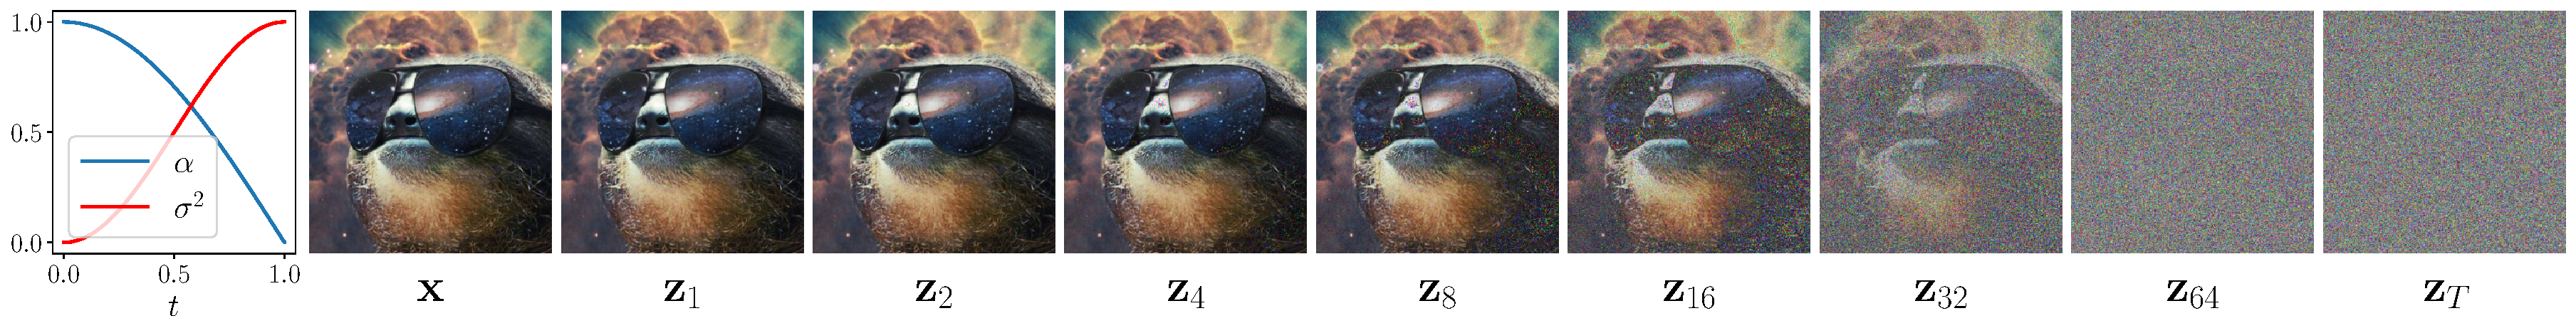
\includegraphics[trim=0 0 0 0,clip,width=\textwidth]{figures/cosine_sloth.pdf}
        \label{fig:cosine_sloth}
    \end{subfigure}
    \\[-8pt]
    \begin{subfigure}{\textwidth}
        \centering 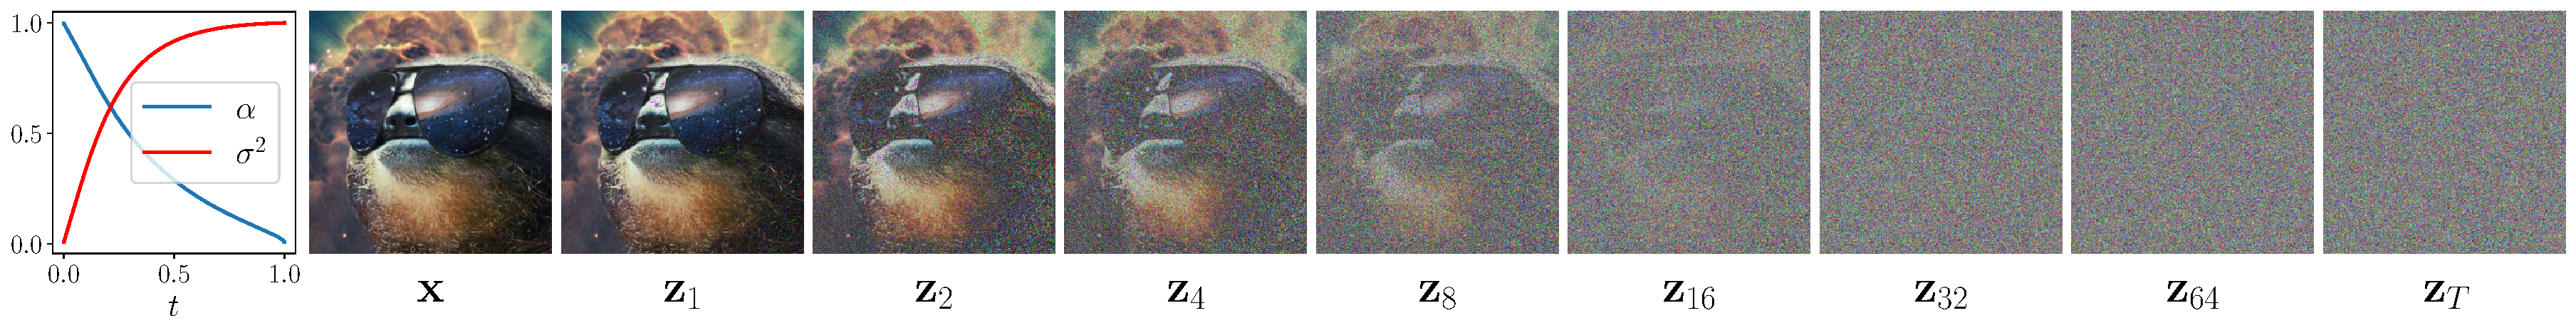
\includegraphics[trim=0 0 0 0,clip,width=\textwidth]{figures/edm_sloth.pdf}
        \label{fig:edm_sloth}
    \end{subfigure}
    \vspace{-20pt}
    \caption{Gaussian diffusion process ($T{=}100$). Showing two popular noise schedules in terms of $\alpha$, $\sigma^2$ as per Section~\ref{subsec: Gaussian Diffusion Process: Forward Time}: (top) cosine~\citep{nichol2021improved}; (bottom) EDM~\citep{karras2022elucidating}.}
    \label{fig: diff_sloth}
\end{figure}
%
\subsection{Forward Process: Gaussian Diffusion}
\label{subsec: Gaussian Diffusion Process: Forward Time}
%
A \textit{Gaussian diffusion process} gradually transforms data $\mathbf{x}$ into random noise by adding increasing amounts of Gaussian noise at each timestep $t=0,\dots,1$ resulting in a set of latent variables $\mathbf{z}_0,\dots,\mathbf{z}_1$.\footnote{For consistency with the continuous-time case where $T \to \infty$, we denote the latent variables as $\mathbf{z}_{0:1}$ rather than $\mathbf{z}_{1:T}$.}
Each latent variable $\mathbf{z}_t$ is simply a noisy version of $\mathbf{x}$, and its distribution conditional on $\mathbf{x}$ is given by:
%
\begin{align}
    && q(\mathbf{z}_t \mid \mathbf{x}) = \mathcal{N}\left(\mathbf{z}_t;\alpha_{t} \mathbf{x}, \sigma^2_{t} \mathbf{I}\right), && \mathbf{z}_t = \alpha_{t} \mathbf{x} + \sigma_{t}\boldsymbol{\epsilon}_t, && \boldsymbol{\epsilon}_t \sim \mathcal{N}\left(\boldsymbol{\epsilon}_t; 0, \mathbf{I}\right),&&
\end{align}
%
where $\alpha_{t} \in (0,1)$ and $\sigma^2_{t} \in (0,1)$ are chosen scalar valued functions of time $t \in [0,1]$. See Figures~\ref{fig: gd},~\ref{fig: diff_sloth}.

The key idea is to define the forward diffusion process such that the noisiest latent variable $\mathbf{z}_1$ at time $t=1$ is standard Gaussian distributed: $q(\mathbf{z}_1 \mid \mathbf{x}) = \mathcal{N}(\mathbf{z}_1; 0, \mathbf{I})$, thus $q(\mathbf{z}_1 \mid \mathbf{x}) = q(\mathbf{z}_1)$. To that end, the scaling coefficients $\alpha_{0} > \ldots > \alpha_{1}$ \textit{decrease} w.r.t. time $t$, whereas the noise variances $\sigma_{0}^2 < \ldots < \sigma_{1}^2$ \textit{increase} w.r.t. $t$. As we will show, this enables us to learn a generative Markov chain which starts from $\mathbf{z}_1 \sim q(\mathbf{z}_1)$ and reverses the forward diffusion process to obtain samples from the data distribution. The implications of this are profound; the \textit{aggregate} posterior $q(\mathbf{z}_1)$ is equal to the prior $p(\mathbf{z}_1)$ by construction, which circumvents the \textit{hole problem} in VAEs (see Figure~\ref{fig: hole}).~\cite{hoffman2016elbo} showed that the optimal prior is the aggregate posterior, as long as our posterior approximation is good enough.

A \textit{variance-preserving} process is achieved by solving for the value of $\alpha_t$ such that the variance of the respective latent variable $\mathbb{V}[\mathbf{z}_t]$ is equal to the variance of the input data $\mathbb{V}[\mathbf{x}]$. This can be important from a modelling perspective, as adding increasing amounts of noise to the input alters its statistics.

We can first apply some basic properties of \textit{variance} to simplify $\mathbb{V}[\mathbf{z}_t]$ as follows:
%
\begin{align}
    \mathbb{V}[\mathbf{z}_t] = \mathbb{V}[\alpha_{t} \mathbf{x} + \sigma_{t}\boldsymbol{\epsilon}_t] = \mathbb{V}[\alpha_{t} \mathbf{x}] + \mathbb{V}[\sigma_{t}\boldsymbol{\epsilon}_t] = \alpha_{t}^2\mathbb{V}[\mathbf{x}] + \sigma_{t}^2\mathbb{V}[\boldsymbol{\epsilon}_t] = \alpha_{t}^2\mathbb{V}[\mathbf{x}] + \sigma_{t}^2,
\end{align}
%
since $\mathbb{V}[\boldsymbol{\epsilon}_t] = 1$ by definition. Taking the result and solving for $\alpha_t$ yields
%
\begin{align}
    \alpha_{t}^2\mathbb{V}[\mathbf{x}] + \sigma_{t}^2 & = \mathbb{V}[\mathbf{x}] 
    \\[2pt] \alpha_{t}^2 & = \frac{\mathbb{V}[\mathbf{x}] - \sigma_{t}^2}{\mathbb{V}[\mathbf{x}]}
    \\[2pt] \implies \mathbb{V}[\mathbf{z}_t] & = \mathbb{V}[\mathbf{x}] \iff \alpha_{t}^2 = 1 - \frac{\sigma_{t}^2}{\mathbb{V}[\mathbf{x}]},
\end{align}
%
which further simplifies to $\alpha_t^2 = 1 - \sigma_t^2$ as long as our input data is standardized.
%
\newpage
\subsubsection{Linear Gaussian Transitions: $q(\mathbf{z}_t \mid \mathbf{z}_{s})$}
\label{subsubsec: lgt}
The conditional distribution of $\mathbf{z}_t$ given a preceding latent variable $\mathbf{z}_s$, for any timestep $s < t$, is:
%
\begin{align}
    &&q(\mathbf{z}_t \mid \mathbf{z}_{s}) = \mathcal{N}\left(\mathbf{z}_t;\alpha_{t|s}\mathbf{z}_s, \sigma_{t|s}^2 \mathbf{I} \right), && \mathbf{z}_t = \alpha_{t|s} \mathbf{z}_s + \sigma_{t|s}\boldsymbol{\epsilon}_t, && \boldsymbol{\epsilon}_t \sim \mathcal{N}\left(\boldsymbol{\epsilon}_t; 0, \mathbf{I}\right),&&
\end{align}
%
which forms a Markov chain: $\mathbf{z}_1 \leftarrow \mathbf{z}_{(T-1)/T} \leftarrow \mathbf{z}_{(T-2)/T} \leftarrow \cdots \leftarrow \mathbf{z}_0 \leftarrow \mathbf{x}$, see Figure~\ref{fig: mt} for an example. In the continuous-time case where $T \to \infty$, each transition is w.r.t. an infinitesimal change in time $\mathrm{d}t$.

The transition distribution $q(\mathbf{z}_t \mid \mathbf{z}_{s})$ is useful for computing closed-form expressions for the parameters of the posterior $q(\mathbf{z}_s \mid \mathbf{z}_t, \mathbf{x})$, which defines our \textit{reverse-process}, i.e. the generative model (ref. Section~\ref{subsubsec: qzs}).
% To remain consistent with prior work and simplify notation, we may use the same symbols to denote random variables and their outcomes whenever our intentions can be clearly understood from context.

Let's focus on deriving $\alpha_{t|s}$ first. By construction, we know that each $\mathbf{z}_t$ is given by:
%
\begin{align}
    \mathbf{z}_t = \alpha_{t} \mathbf{x} + \sigma_{t}\boldsymbol{\epsilon}_t = \alpha_{t} \left(\frac{\mathbf{z}_s - \sigma_s \boldsymbol{\epsilon}_s}{\alpha_s} \right) + \sigma_{t}\boldsymbol{\epsilon}_t,
\end{align}
%
since $\mathbf{x} = (\mathbf{z}_s - \sigma_s \boldsymbol{\epsilon}_s) / \alpha_s$ for any $s<t$. The conditional mean of $q(\mathbf{z}_t \mid \mathbf{z}_{s})$ is then readily given by:
\begin{align}
    \mathbb{E} \left[ \mathbf{z}_t \mid \mathbf{z}_s \right] &= \alpha_{t} \left(\frac{\mathbf{z}_s - \sigma_s \mathbb{E} \left[\boldsymbol{\epsilon}_s\right]}{\alpha_s} \right) + \sigma_{t}\mathbb{E} \left[\boldsymbol{\epsilon}_t\right] 
    \\[5pt] &
    = \frac{\alpha_t}{\alpha_s}\mathbf{z}_s \customtag{since $\mathbb{E}[\boldsymbol{\epsilon}_t] = 0, \ \forall t$}
    \\[5pt] & 
    \eqqcolon \alpha_{t|s}\mathbf{z}_s. \label{eq: cond_alpha}
\end{align}
%
To compute a closed-form expression for the variance $\sigma^2_{t|s}$ of the transition distribution $q(\mathbf{z}_t \mid \mathbf{z}_{s})$, we can start by rewriting the equation for $\mathbf{z}_t$ in terms of the preceding latent $\mathbf{z}_s$ as follows:
%
\begin{align}
    \mathbf{z}_t &= \alpha_{t|s} \mathbf{z}_s + \sigma_{t|s}\boldsymbol{\epsilon}_{t} 
    \\[5pt] &= \frac{\alpha_{t}}{\alpha_{s}} \left( \alpha_s \mathbf{x} + \sigma_s \boldsymbol{\epsilon}_s\right) + \sigma_{t|s}\boldsymbol{\epsilon}_{t} \customtag{substitute $\alpha_{t|s}$ and $\mathbf{z}_s$}
    \\[5pt] & = \alpha_t \mathbf{x} + \frac{\alpha_t}{\alpha_s} \sigma_s \boldsymbol{\epsilon}_s + \sigma_{t|s}\boldsymbol{\epsilon}_{t}    
    \\[5pt] \implies \sigma_t \boldsymbol{\epsilon}_{t} & = \frac{\alpha_t}{\alpha_s} \sigma_s \boldsymbol{\epsilon}_s + \sigma_{t|s}\boldsymbol{\epsilon}_{t}. \customtag{since $\mathbf{z}_t = \alpha_t \mathbf{x} + \sigma_t \boldsymbol{\epsilon}_t$}
\end{align}
%

The above implication allows us to compute the variance $\sigma_{t|s}^2$ straightforwardly. Firstly, recall that variance is invariant to changes in a location parameter, therefore: $\mathbb{V}\left[ cX \right] = c^2\mathbb{V}\left[ X \right]$ for some constant $c$ and random variable $X$. Secondly, the variance of a sum of $n$ independent random variables is simply the sum of their variances: $\mathbb{V}\left[\sum_{i=1}^n X_n\right] = \sum_{i=1}^n\mathbb{V}\left[ X_i\right]$. Using these two properties we can show that:
%
\begin{align}
    \mathbb{V}\left[\sigma_t \boldsymbol{\epsilon}_t\right] & = \mathbb{V}\left[\frac{\alpha_t}{\alpha_s} \sigma_s \boldsymbol{\epsilon}_s + \sigma_{t|s}\boldsymbol{\epsilon}_{t}\right]
    \\[5pt] \sigma^2_t\mathbb{V}\left[ \boldsymbol{\epsilon}_t\right] & = \left(\frac{\alpha_t}{\alpha_s}\right)^2 \sigma_s^2\mathbb{V}\left[ \boldsymbol{\epsilon}_s\right] + \sigma_{t|s}^2 \mathbb{V}\left[\boldsymbol{\epsilon}_{t}\right]
    \\[5pt] \sigma^2_t & = \left(\frac{\alpha_t}{\alpha_s}\right)^2 \sigma_s^2 + \sigma_{t|s}^2
    \\[5pt] \sigma_{t|s}^2 & = \sigma^2_t - \alpha_{t|s}^2 \sigma_s^2. \label{eq: post_var}
\end{align}
%
\subsubsection{Top-down Posterior: $q(\mathbf{z}_s \mid \mathbf{z}_{t}, \mathbf{x})$}
\label{subsubsec: qzs}
Since the forward process is a Markov chain, the joint distribution of any two latent variables $\mathbf{z}_t$ and $\mathbf{z}_s$ where $t > s$ factorizes as: $q(\mathbf{z}_s, \mathbf{z}_t \mid \mathbf{x}) =
q(\mathbf{z}_t \mid \mathbf{z}_s)q(\mathbf{z}_s \mid \mathbf{x})$. Using Bayes' theorem, it is then possible to derive closed-form expressions for the parameters of the posterior distribution $q(\mathbf{z}_s \mid \mathbf{z}_{t}, \mathbf{x})$, which is itself Gaussian due to conjugacy, where $q(\mathbf{z}_s \mid \mathbf{x})$ acts as a Gaussian prior and $q(\mathbf{z}_t \mid \mathbf{z}_s)$ a Gaussian likelihood:
%
\begin{align}
    &&q(\mathbf{z}_s \mid \mathbf{z}_{t}, \mathbf{x}) = \mathcal{N} \left(\mathbf{z}_s;\boldsymbol{\mu}_Q(\mathbf{z}_t, \mathbf{x}; s, t), \sigma^2_Q(s,t) \mathbf{I}\right), && \mathbf{z}_s = \boldsymbol{\mu}_Q(\mathbf{z}_t, \mathbf{x}; s, t) + \sigma_{Q}(s,t)\boldsymbol{\epsilon}_t, &&
\end{align}
%
with $\boldsymbol{\epsilon}_t \sim \mathcal{N}\left(\boldsymbol{\epsilon}_t; 0, \mathbf{I}\right)$. In the following, we will derive closed-form expressions for the posterior parameters $\boldsymbol{\mu}_Q(\mathbf{z}_t, \mathbf{x}; s, t)$ and $\sigma^2_Q(s,t)$ in detail. For a graphical model of the posterior see Figure~\ref{fig: tdp}.

Before proceeding, we note that this posterior distribution will be instrumental in defining our generative model (i.e. the reverse process) as explained later on in Section~\ref{subsec: Discrete-time Generative Model}. Furthermore, notice that the posterior $q(\mathbf{z}_s \mid \mathbf{z}_t, \mathbf{x})$ coincides with the \textit{top-down} inference model specification of a hierarchical VAE. 

For simplicity, let $D$ denote the dimensionality of $\mathbf{z}_t$, satisfying $\mathrm{dim}(\mathbf{z}_t) = \mathrm{dim}(\mathbf{x}), \forall t$. Furthermore, recall that our covariance matrix of choice is isotropic/spherical: $\sigma^2_Q \mathbf{I}$. The posterior is then given by
%
\begin{align}
    q(\mathbf{z}_s \mid \mathbf{z}_t, \mathbf{x}) &
    = \frac{q(\mathbf{z}_t \mid \mathbf{z}_s)q(\mathbf{z}_s \mid \mathbf{x})}{q(\mathbf{z}_t \mid \mathbf{x})} 
    \\ & \propto q(\mathbf{z}_t \mid \mathbf{z}_s)q(\mathbf{z}_s \mid \mathbf{x})
    \\[5pt] & 
    = \mathcal{N}\left(\mathbf{z}_t; \alpha_{t|s} \mathbf{z}_s, \sigma^2_{t|s}\mathbf{I}\right)\cdot \mathcal{N}\left(\mathbf{z}_s;\alpha_s\mathbf{x}, \sigma^2_s\mathbf{I} \right)
    \\[5pt] & = \prod_{i=1}^D \frac{1}{\sigma_{t|s}\sqrt{2\pi}}\exp\left\{-\frac{1}{2\sigma_{t|s}^2}\left(\mathbf{z}_{t,i} - \alpha_{t|s}\mathbf{z}_{s,i}\right)^2 \right\} \cdot \prod_{i=1}^D \frac{1}{\sigma_{s}\sqrt{2\pi}}\exp\left\{-\frac{1}{2\sigma^2_{s}}\left(\mathbf{z}_{s,i} - \alpha_{s}\mathbf{x}_i\right)^2 \right\} 
    \\[5pt] & \propto \prod_{i=1}^D \exp\left\{-\frac{1}{2\sigma_{t|s}^2}\left(\mathbf{z}_{t,i} - \alpha_{t|s}\mathbf{z}_{s,i}\right)^2 \right\} \cdot \prod_{i=1}^D \exp\left\{-\frac{1}{2\sigma^2_{s}}\left(\mathbf{z}_{s,i} - \alpha_{s}\mathbf{x}_i\right)^2 \right\}
    \\[5pt] & = \prod_{i=1}^D \exp\left\{-\frac{1}{2\sigma^2_{t|s}}\left(\mathbf{z}_{t,i}^2 - 2\mathbf{z}_{t,i}\alpha_{t|s}\mathbf{z}_{s,i} + \alpha_{t|s}^2\mathbf{z}_{s,i}^2\right) -\frac{1}{2\sigma^2_{s}}\left(\mathbf{z}_{s,i}^2 - 2\mathbf{z}_{s,i}\alpha_{s}\mathbf{x}_i + \alpha_{s}^2\mathbf{x}_i^2\right) \right\}
    \\[5pt] & = \prod_{i=1}^D \exp\left\{-\frac{1}{2}\left[\frac{\mathbf{z}_{t,i}^2 - 2\mathbf{z}_{t,i}\alpha_{t|s}\mathbf{z}_{s,i} + \alpha_{t|s}^2\mathbf{z}_{s,i}^2}{\sigma^2_{t|s}} + \frac{\mathbf{z}_{s,i}^2  -2\mathbf{z}_{s,i}\alpha_{s}\mathbf{x}_i + \alpha_{s}^2\mathbf{x}_i^2}{\sigma^2_{s}} \right]\right\}
    \\[5pt] & = \prod_{i=1}^D \exp\left\{-\frac{1}{2}\left[
    \mathbf{z}_{s,i}^2\left(\frac{\alpha_{t|s}^2}{\sigma_{t|s}^2} + \frac{1}{\sigma_s^2}\right) -2\mathbf{z}_{s,i}\left( \frac{\alpha_{t|s}\mathbf{z}_{t,i}}{\sigma_{t|s}^2}+\frac{\alpha_s\mathbf{x}_i}{\sigma_s^2}\right)
    +\frac{\mathbf{z}_{t,i}^2}{\sigma_{t|s}^2} + \frac{\alpha_s^2\mathbf{x}_i^2}{\sigma_{s}^2}
    \right]\right\}. 
    \label{eq:mm}
\end{align}
%

The next step is to `match the moments' from Equation~\eqref{eq:mm} with what we expect to see in a Gaussian distribution, i.e. something of the form: $\mathcal{N}\left(x;\mu, \sigma^2 \right)\propto \exp\left\{- \frac{x^2}{2\sigma^2} + \frac{\mu x}{\sigma^2} - \frac{\mu^2}{2\sigma_2}
 \right\}$. This exercise yields closed-form expressions for the parameters of the posterior distribution as desired. Without loss of generality, consider the $D=1$ dimensional case for brevity.
  
 Matching the first term in Eq.~\eqref{eq:mm} with $-\frac{x^2}{2\sigma^2}$ we can see that:
%
\begin{align}
    -\frac{\mathbf{z}_s^2}{2}\left(\frac{\alpha_{t|s}^2}{\sigma_{t|s}^2} + \frac{1}{\sigma_s^2}\right) \implies \frac{1}{\sigma^2_Q} = \frac{\alpha_{t|s}^2}{\sigma_{t|s}^2} + \frac{1}{\sigma_s^2},
\end{align}
%
where $\sigma^2_Q$ is the variance of the posterior $q(\mathbf{z}_s \mid \mathbf{z}_t, \mathbf{x})$. Matching the second term in Eq.~\eqref{eq:mm} with $\frac{\mu x}{\sigma^2}$ we get:
%
\begin{align}
    \mathbf{z}_s\left(\frac{\alpha_{t|s}\mathbf{z}_t}{\sigma_{t|s}^2} + \frac{\alpha_s\mathbf{x}}{\sigma_s^2}\right) \implies \frac{\boldsymbol{\mu}_Q}{\sigma^2_Q} = \frac{\alpha_{t|s}\mathbf{z}_t}{\sigma_{t|s}^2} + \frac{\alpha_s\mathbf{x}}{\sigma_s^2} \implies \boldsymbol{\mu}_Q = {\sigma^2_Q} \left(\frac{\alpha_{t|s}\mathbf{z}_t}{\sigma_{t|s}^2} + \frac{\alpha_s\mathbf{x}}{\sigma_s^2}\right),
\end{align}
where $\boldsymbol{\mu}_Q$ is the mean of the posterior $q(\mathbf{z}_s \mid \mathbf{z}_t, \mathbf{x})$. 

The closed-form expressions for $\boldsymbol{\mu}_Q$, $\sigma^2_Q$ simplify quite significantly:
\begin{align}
    \frac{1}{\sigma^2_Q} &= \frac{\sigma^2_s}{\sigma^2_s}\cdot
    \frac{\alpha_{t|s}^2}{\sigma_{t|s}^2} + \frac{\sigma^2_{t|s}}{\sigma^2_{t|s}} \cdot \frac{1}{\sigma_s^2} \\[5pt] & = \frac{\alpha_{t|s}^2 \sigma_s^2 + \sigma_{t|s}^2}{\sigma_{t|s}^2\sigma_s^2} \implies \sigma_Q^2 = \frac{\sigma_{t|s}^2\sigma_s^2}{\alpha_{t|s}^2 \sigma_s^2 + \sigma_{t|s}^2},
\end{align}
%
and for the posterior mean we then have:
\begin{align}
    \boldsymbol{\mu}_Q & = 
    {\sigma^2_Q} \left(\frac{\alpha_{t|s}\mathbf{z}_t}{\sigma_{t|s}^2} + \frac{\alpha_s\mathbf{x}}{\sigma_s^2}\right)
    \\[5pt] &= \frac{\sigma_{t|s}^2\sigma_s^2}{\alpha_{t|s}^2 \sigma_s^2 + \sigma_{t|s}^2} \cdot \frac{\sigma_s^2\alpha_{t|s}\mathbf{z}_t + \sigma_{t|s}^2\alpha_s\mathbf{x}}{\sigma_{t|s}^2\sigma_s^2} 
    \\[5pt] &
    = \frac{\sigma_s^2\alpha_{t|s}\mathbf{z}_t + \sigma_{t|s}^2\alpha_s\mathbf{x}}{\alpha_{t|s}^2 \sigma_s^2 + \sigma_{t|s}^2}
    \\[5pt] &= \frac{\alpha_{t|s}\sigma_s^2}{\alpha_{t|s}^2 \sigma_s^2 + \sigma_{t|s}^2}\mathbf{z}_t + \frac{\alpha_s \sigma^2_{t|s}}{\alpha_{t|s}^2 \sigma_s^2 + \sigma_{t|s}^2}\mathbf{x}.
\end{align}
%
Using the fact that $\sigma_{t|s}^2 = \sigma^2_t - \alpha_{t|s}^2 \sigma_s^2$ as in Equation~\ref{eq: post_var}, we get the final expression:
%
\begin{align}
    \boldsymbol{\mu}_Q(\mathbf{z}_t, \mathbf{x};s,t) = \frac{\alpha_{t|s}\sigma_s^2}{\sigma^2_{t}}\mathbf{z}_t + \frac{\alpha_s \sigma^2_{t|s}}{\sigma_{t}^2}\mathbf{x}, \label{eq: post_mu}
\end{align}
%
revealing that the posterior mean $\boldsymbol{\mu}_Q$, equivalently denoted as $\boldsymbol{\mu}_Q(\mathbf{z}_t, \mathbf{x};s,t)$ by~\cite{kingma2021variational}, is essentially a weighted average of the conditioning set $\{\mathbf{z}_t, \mathbf{x}\}$ of the posterior distribution $q(\mathbf{z}_s \mid \mathbf{z}_t, \mathbf{x})$.

In summary, the top-down posterior distribution is given by:
%
\begin{align}
    q(\mathbf{z}_s \mid \mathbf{z}_{t}, \mathbf{x}) & = \mathcal{N} \left(\mathbf{z}_s;\frac{\alpha_{t|s}\sigma_s^2}{\sigma^2_{t}}\mathbf{z}_t + \frac{\alpha_s \sigma^2_{t|s}}{\sigma_{t}^2}\mathbf{x}, \frac{\sigma_{t|s}^2\sigma_s^2}{\alpha_{t|s}^2 \sigma_s^2 + \sigma_{t|s}^2} \mathbf{I}\right)
    \\[5pt] & = \mathcal{N} \left(\mathbf{z}_s;\boldsymbol{\mu}_Q(\mathbf{z}_t, \mathbf{x}; s, t), \sigma^2_Q(s,t) \mathbf{I}\right).
\end{align}
%
To conclude, Table~\ref{tab: dist_params} provides a concise breakdown of all the distributions involved in defining a Gaussian diffusion, along with the respective closed-form expressions of their parameters.

%
\newpage
\begin{table}[!t]
    \centering
    \begin{tabular}{lll}
        \toprule
        Distribution & Mean & Covariance \\
        \midrule
        $q(\mathbf{z}_t \mid \mathbf{x})$ (\S\ref{subsec: Gaussian Diffusion Process: Forward Time})&  $\alpha_t \mathbf{x}$ &  $\sigma_t^2\mathbf{I}$ \\[2pt]
        $q(\mathbf{z}_t \mid \mathbf{z}_s)$ (\S\ref{subsubsec: lgt}) & $\alpha_{t|s} \mathbf{z}_s$ & $\sigma_{t|s}^2\mathbf{I}$ \\[2pt]
        $q(\mathbf{z}_s \mid \mathbf{z}_t, \mathbf{x})$ (\S\ref{subsubsec: qzs}) & $\boldsymbol{\mu}_Q(\mathbf{z}_t, \mathbf{x}; s, t)$ &  $\sigma^2_Q(s,t)\mathbf{I}$ \\[2pt]
        \bottomrule
    \end{tabular}
    \hspace{20pt}
    \begin{tabular}{ll}
        \toprule
        Parameter & Expression \\
        \midrule
        $\alpha_{t|s}$ & $\alpha_t / \alpha_s$ \\[5pt]
        $\sigma^2_{t|s}$ & $\sigma^2_t - \alpha_{t|s}^2 \sigma_s^2$ \\[5pt]
        $\boldsymbol{\mu}_Q(\mathbf{z}_t, \mathbf{x}; s, t)$ & $\displaystyle\frac{\alpha_{t|s}\sigma_s^2}{\sigma^2_{t}}\mathbf{z}_t + \frac{\alpha_s \sigma^2_{t|s}}{\sigma_{t}^2}\mathbf{x}$ \\[5pt]
        $\sigma^2_Q(s,t)$ & $\displaystyle \frac{\sigma_{t|s}^2\sigma_s^2}{\alpha_{t|s}^2 \sigma_s^2 + \sigma_{t|s}^2}$ \\[5pt]
        \bottomrule
    \end{tabular}
    \caption{Breakdown of the distributions involved in defining a typical Gaussian diffusion (LHS), along with closed-form expressions for their respective parameters (RHS). Note that $s$ denotes a preceding timestep relative to timestep $t$, i.e. $s < t$. The top-down posterior distribution $q(\mathbf{z}_s \mid \mathbf{z}_t, \mathbf{x})$ is tractable due to Gaussian conjugacy: $q(\mathbf{z}_s \mid \mathbf{z}_t, \mathbf{x}) \propto q(\mathbf{z}_t \mid \mathbf{z}_s) q(\mathbf{z}_s \mid \mathbf{x}) $, where $q(\mathbf{z}_s \mid \mathbf{x})$ plays the role of a conjugate (Gaussian) prior and $q(\mathbf{z}_t \mid \mathbf{z}_s)$ the plays the role of a Gaussian likelihood.}
    \label{tab: dist_params}
\end{table}
\subsubsection{Learning the Noise Schedule}
\label{subsubsec: Noise Schedule}
%
Perturbing data with multiple noise scales and choosing an appropriate \textit{noise schedule} is instrumental to the success of diffusion models. The noise schedule of the forward process is typically pre-specified and has no learnable parameters, however, VDMs learn the noise schedule via the parameterization:
%
\begin{align}
    \sigma_t^2 = \mathrm{sigmoid}\left(\gamma_{\boldsymbol{\eta}}(t)\right),
\end{align}
%
where $\gamma_{\boldsymbol{\eta}}(t)$ is a \textit{monotonic} neural network comprised of linear layers with weights $\boldsymbol{\eta}$ restricted to be positive. A monotonic function is a function defined on a subset of the real numbers which is either entirely non-increasing or entirely non-decreasing. As explained later, the noise schedule can be conveniently parameterized in terms of the signal-to-noise ratio. The signal-to-noise ratio (SNR) is defined as $\mathrm{SNR}(t) = \alpha_t^2 / \sigma_t^{2}$, and since $\mathbf{z}_t$ grow noisier over time we have that: $\mathrm{SNR}(t) < \mathrm{SNR}(s)$ for any $t > s$. 

For now, we provide some straightforward derivations of the expressions for $\alpha_t^2$ and $\mathrm{SNR}(t)$ as a function of $\gamma_{\boldsymbol{\eta}}(t)$. Recall that in a variance-preserving diffusion process $\alpha_t^2 = 1 - \sigma_t^2$, therefore:
%
\begin{align}
     \alpha_t^2 &= 1- \sigma_t^2 = 1 - \mathrm{sigmoid}\left(\gamma_{\boldsymbol{\eta}}(t)\right) \implies \alpha_t^2 = \mathrm{sigmoid}\left(-\gamma_{\boldsymbol{\eta}}(t)\right),
\end{align}
%
as for an input $x \in \mathbb{R}$ the following holds 
%
\begin{align}
     1 - \mathrm{sigmoid}\left(x\right) &= 1 - \frac{1}{1 + e^{-x}} = \frac{1 + e^{-x}}{1 + e^{-x}} - \frac{1}{1 + e^{-x}} = \frac{e^{-x}}{1 + e^{-x}} \cdot \frac{e^{x}}{e^{x}} 
     % \\[5pt] &
     = \mathrm{sigmoid}\left(-x\right).
\end{align}
%
To derive $\mathrm{SNR}(t)$ as a function of $\gamma_{\boldsymbol{\eta}}(t)$, we simply substitute in the above equations and simplify:
%
\begin{align}
    \mathrm{SNR}(t) &= \frac{\alpha_t^2}{\sigma_t^2} = \frac{\mathrm{sigmoid}\left(-\gamma_{\boldsymbol{\eta}}(t)\right)}{\mathrm{sigmoid}\left(\gamma_{\boldsymbol{\eta}}(t)\right)} \customtag{by definition}
    \\[5pt] &= \frac{(1+e^{\gamma_{\boldsymbol{\eta}}(t)})^{-1}}{(1+e^{-\gamma_{\boldsymbol{\eta}}(t)})^{-1}} = \frac{1+e^{-\gamma_{\boldsymbol{\eta}}(t)}}{1+e^{\gamma_{\boldsymbol{\eta}}(t)}} = \frac{\frac{e^{\gamma_{\boldsymbol{\eta}}(t)}}{e^{\gamma_{\boldsymbol{\eta}}(t)}}+\frac{1}{e^{\gamma_{\boldsymbol{\eta}}(t)}
    }}{1+e^{\gamma_{\boldsymbol{\eta}}(t)}} \cdot \frac{e^{\gamma_{\boldsymbol{\eta}}(t)}}{e^{\gamma_{\boldsymbol{\eta}}(t)}} = \frac{e^{\gamma_{\boldsymbol{\eta}}(t)}+1}{e^{\gamma_{\boldsymbol{\eta}}(t)}(1+e^{\gamma_{\boldsymbol{\eta}}(t)})}
    \\[5pt] &
    = \frac{1}{e^{\gamma_{\boldsymbol{\eta}}(t)}}, \label{eq: snrt}
\end{align}
%
which is equivalently expressed as $\mathrm{SNR}(t) = \mathrm{exp}(-\gamma_{\boldsymbol{\eta}}(t))$.